\nnsec{Results}
%\nnsub{Two-Choice Rule Switching Task}
Eighteen adult male mice were trained to high proficiency on a two-choice sensorimotor decision making task under head fixation (Fig. \ref{fig:Fig1}A--B). The task consisted of a set of trials in which subjects could choose between two stainless steel water spouts placed on either side of the mouth, only one of which (the target) would provide a water reward when chosen. A sound cue presented at the start of each trial---either an upsweep or downsweep---indicated the target side (left for upsweeps, right for downsweeps).

\begin{figure}[htbp]

\begin{center}
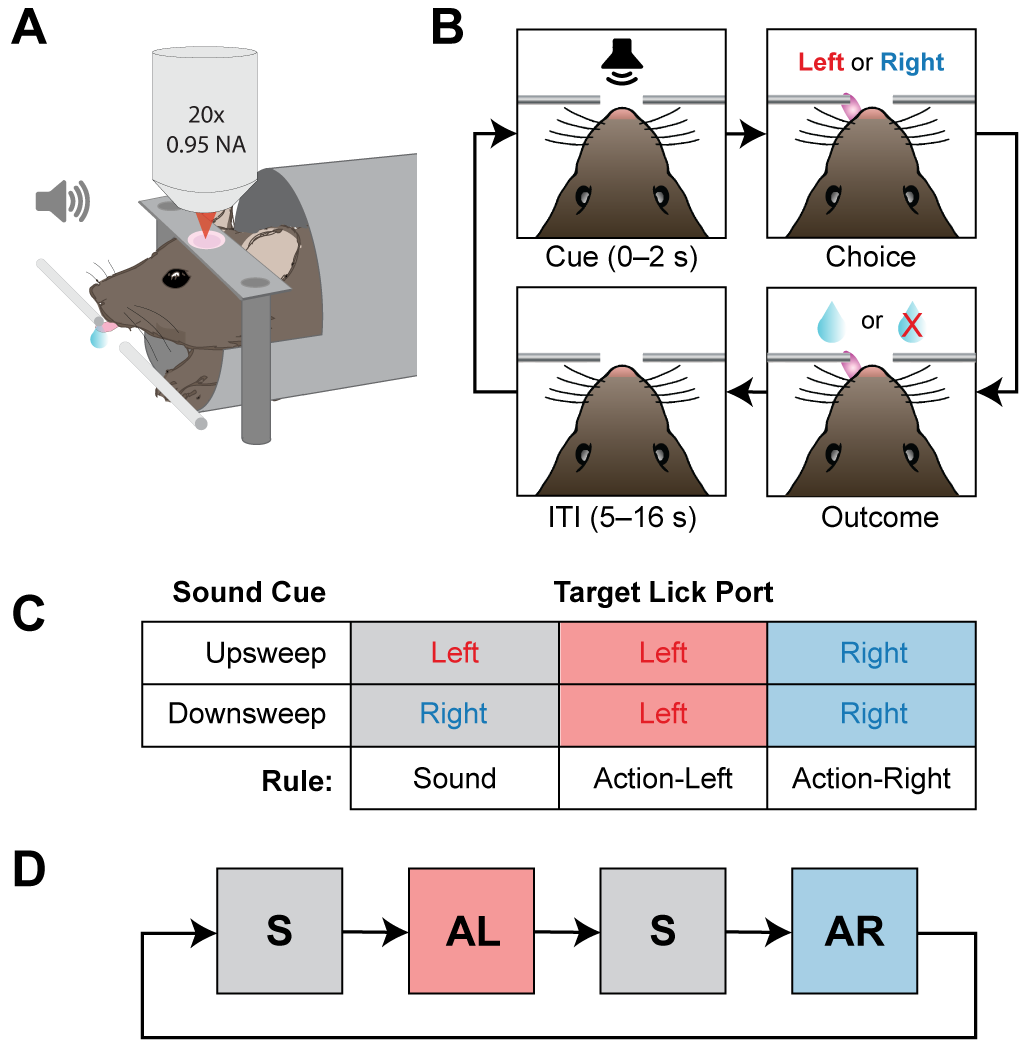
\includegraphics[width=8.7cm]{Figures/Chapter4/Fig1}
\end{center}

\caption[Rule switching task for head-fixed mice]
{Rule switching task for head fixed mice. (A) Experimental setup for two-choice sensorimotor task with simultaneous two-photon imaging. Mice rested inside of a stainless steel tube, with the head immobilized using a cranial implant. Two water spouts were placed on either side of the mouth to deliver rewards. (B) Flow diagram of trial structure. A sound cue was played at the start of each trial, indicating the target spout that would be rewarded (left or right). To obtain the reward, subjects were required to lick the target within 2 s following cue onset. After a random intertrial interval (ITI) of 5--16 s, a new sound cue was presented, providing a fresh opportunity to lick for a reward. (C) Table indicating the target spout signified by each sound cue in each rule context. (D) Flow diagram of session structure. Trials governed by each rule were organized into blocks. Sound blocks (S) were interleaved with action blocks that alternated between the action-left (AL) and action-right (AR) rule. A new rule block was initiated on the next trial after an accuracy criterion was met (85\% for the past 20 trials of the current block).}

\label{fig:Fig1}
\end{figure}

Subjects were immediately rewarded with $\sim$ 2 \si{\uL} of water if the target spout was chosen within 2 s of cue onset (a hit). Choosing the non-target spout (an error) resulted in playback of a mild white noise sound. After a random interval of 5--16 seconds, the next cue was played, providing the opportunity to make another choice. New trials were generated until the subject failed to respond (missed) for twenty consecutive trials.

After meeting a performance criterion (three consecutive sessions at $>85\%$  accuracy), subjects were challenged with a modified version of this task, which was designed to elicit flexible sensorimotor decisions. Namely, the fixed relationship between each sound cue and its corresponding target was replaced with three alternative rules for action selection (Fig. \ref{fig:Fig1}C). 

In the sound rule, upsweeps signified a left target, and downsweeps signified a right target as described above. In the action-left rule, the target on every trial was the left spout, regardless of whether upsweeps or downsweeps were presented. Conversely, under the action-right rule, the right spout was always the target, irrespective of the auditory cue. 

Sessions were structured into alternating blocks of sound and action trials, such that each rule was enforced for at least 20 trials at a time (Fig. \ref{fig:Fig1}D). After 20 consecutive trials with $\geq 85\%$  accuracy, a rule-switch would occur---ie, a new rule block would begin on the next trial.

Subjects participated in $4 \pm 0$ sessions each (range: 2--5; $N=18$ mice), for a total of 64 sessions. Within each session, they completed an average $6 \pm 0$ rule blocks over the course of $563 \pm 21$ trials (all descriptive statistics are reported as $\mathit{mean}\pm\mathit{SEM}$; unless otherwise noted, the sample size $N$ is given by the number of sessions).

We used two-photon calcium imaging to measure the activity of SST, PV, VIP, and PYR neurons in layer 2/3 of the most dorsal field of the MFC (the secondary motor cortex, M2) while subjects participated in this task. Imaging was restricted to the cell-type of interest in each experiment using one of three approaches. To target GABAergic interneurons (SST, PV, or VIP), we used transgenic mice that selectively express cyclic recombinase (cre) in the cell-type of interest \citep{taniguchi11}. In some cases ($N =$ 5 \emph{SST-cre} and 2 \emph{PV-cre} mice), an adeno-associated virus (AAV) encoding a cre-dependent GCaMP6s construct (AAV1-hSyn-Flex-GCaMP6s-WPRE-SV40) was injected into M2. In other cases, experimental subjects were F1 hybrids produced by crossing the cre-driver line with a second transgenic mouse line, \emph{Ai148} \citep{daigle18}, that expresses GCaMP6f in a cre-dependent manner ($N =$ 5 \emph{VIP-cre;Ai148} mice and 1 \emph{PV-cre;Ai148} mouse). To target pyramidal (PYR) neurons, we injected an AAV that encodes GCaMP6f under control of the CaMKII promoter (AAV1-CaMKII-GCaMP6f-WPRE-SV40; $N = 5$) \citep{kuchibhotla17, ali20}.

We visually identified a total of \num{4993} GCaMP\textsuperscript{+} neurons across all imaging sessions (Supplementary Table \ref{tab:expTable}). After excluding \num{1006} cells in which the baseline fluorescence was dimmer on average than that of the background (see \hyperlink{methods_dFF}{Methods}), we obtained cellular fluorescence time series from a total of 286 SST, 479 VIP, 263 PV, and \num{2959} PYR neurons. On average, $22 \pm 2$ SST, $25 \pm 1$ VIP, $22 \pm 2$ PV, or $148 \pm 9$ PYR neurons were included per session ($N =$ 13, 19, 12, and 20 sessions, respectively). The number of completed rule-blocks per session was similar during recordings from all cell-types, at $6 \pm 0$ for VIP and PYR, $6 \pm 1$ for SST, and $7 \pm 1$ for PV ($F_{3,60}=0.24$, $p=0.87$, 1-way ANOVA). 

\nnsub{Dependence of Lick Output on Task Structure}
As expected, the pattern of licking output was dependent on the task structure. Overall lick density varied based on elapsed time within the trial, as well as trial outcome (Fig. \ref{fig:Fig2}A--B). Specifically, the mean lick rate in completed trials increased from $0.9 \pm 0.1$ Hz in the 2 s prior to cue onset ("pre-cue"), to $2.6 \pm 0.1$ Hz in the 2 s following it ("post-cue"; paired $t_{63} =38.4$, $p=\num{3e-45}$). The mean lick rate post-cue was higher for hits than errors ($1.3 \pm 0.0$ vs. $3.3 \pm 0.1$ Hz; paired $t_{63} =24.2$, $p=\num{2e-33}$),\ which likely reflects differences in consummatory licking.

\begin{figure}[htbp]

\begin{center}
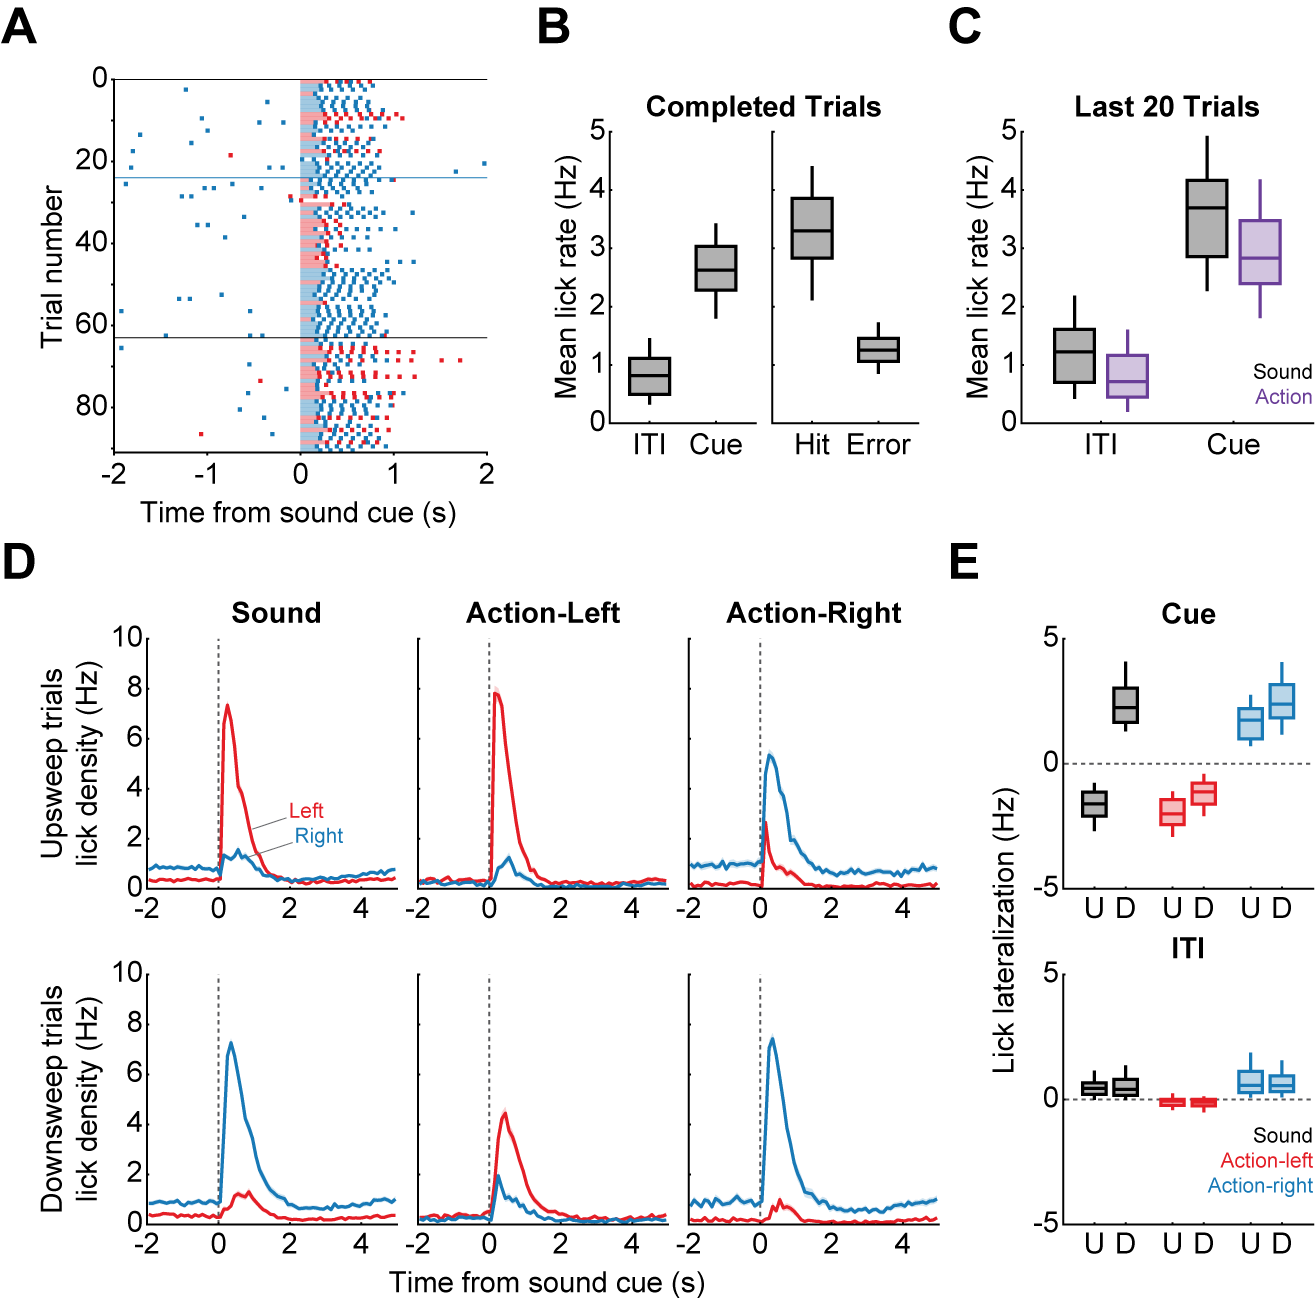
\includegraphics[width=11.4cm]{Figures/Chapter4/Fig2} 
\end{center}

\caption[Dependence of lick output on task structure]
{Dependence of lick output on the task structure. (A) Raster plot of individual lick times, aligned to cue onset during the first three blocks of an example session. Rows of the raster correspond to consecutive trials. The cue period of each trial is highlighted in pale red for upsweeps and pale blue for downsweeps, with red and blue tick marks representing left and right licks, respectively. Fine horizontal lines indicate the first trial of each rule block. The order of the blocks was sound--action-right--sound. (B) Mean lick rates for the 2 s periods before and after cue onset (ITI and Cue, respectively), estimated from all completed trials. Left, overall comparison of ITI and cue periods. Right, comparison of hit and error trials during the cue period. (C) Mean lick rates for the ITI and cue periods, presented separately for sound (black) and action trials (purple). (D) Lick density at the left (red) and right port (blue) across all sessions, calculated in 100 ms time bins surrounding cue onset. Data are plotted separately as the $\mathit{mean} \pm \mathit{SEM}$ for upsweep (top) and downsweep trials (bottom) within each block type. (E) Lick lateralization in upsweep (U) and downsweep trials (D) within each block type. Lick lateralization was calculated as the difference between the number of right and left licks during the 2 s before (bottom) and after cue onset (top) in each trial. Positive and negative values indicate a greater number of right and left licks, respectively. For C--E, analysis was restricted to the last twenty trials of each block: the period in which the accuracy criterion was met. For B--E, $N = 64$ sessions. Box plots in all figures represent quartiles 1--3 for each group. Whiskers indicate the 9th and 91st percentiles.}

\label{fig:Fig2}
\end{figure}


An important difference between sound and action trials is that a conditional mode of action selection \citep{mitz1991learning} is optimal under the sound rule; ie, only under the sound rule should choices depend on the identity of the sound cue. By contrast, the two action rules prescribe an unconditional mode of action selection that does not depend on cue identity. Therefore, in principle, correct choices could be made and even acted upon prior to cue onset in action trials, leading to rule-dependent differences in anticipatory licking.

To examine differences across rule types, we limited our analyses to the last twenty trials of each rule block---the period where at least 85$\%$  of choices were consistent with the corresponding rule. The mean pre-cue lick rate in action trials ($0.9 \pm 0.1$ Hz) was no greater than in sound trials ($1.2 \pm 0.1$ Hz; Fig. \ref{fig:Fig2}C). Moreover, the mean lick rate increased substantially upon cue onset in both sound and action trials (sound: $\Delta=2.4$ Hz, paired $t_{63} =28.7$, $p=\num{2e-38}$; action: $\Delta=2.1$ Hz, paired $t_{63}=29.7$, $p=\num{9e-39}$). Thus, the overall pattern of licking output was largely conserved across rule types, despite fundamental differences in their temporal constraints on action selection (Fig. \ref{fig:Fig2}D).

Sound, action-left, and action-right rules are defined by the instructive content of each sound cue. Specifically, upsweeps and downsweeps signify diverging targets during sound blocks (left vs. right), and convergent but opposing targets during action-left and action-right blocks. Thus, choices should depend on an interaction between cue identity and the current rule. However, the choice made on a given trial concerns only the initial lick following the sound cue. To examine the extent to which the overall pattern of directional licking was structured by the task, we calculated a measure of lick lateralization by subtracting the mean left-lick rate from the mean right-lick rate during the post-cue period of each trial. For example, in sound trials, lick lateralization was $-1.6 \pm 0.1$ Hz following an upsweep, and $2.5 \pm 0.1$ Hz following a downsweep.

We examined the dependence of this measure on cue identity, block-type, and their interaction with a 2-way repeated measures ANOVA  (Fig. \ref{fig:Fig2}E). Individual comparisons were made using Tukey’s post hoc test. As expected, this analysis revealed a significant dependence of lick lateralization on the interaction between block type and cue identity ($F_{2,126}=390$, $p=\num{6e-55}$). Specifically, lick lateralization following upsweeps versus downsweeps differed most during sound blocks ($\Delta=4.1$ Hz, $p=\num{1e-10}$). A much smaller difference was observed during action blocks (action-left: $\Delta=0.8$ Hz, $p=\num{1.1e-10}$; action-right: $\Delta=0.8$ Hz, $p=\num{1.1e-10}$). 

An identical analysis considering the pre-cue period revealed a small but significant difference in lick lateralization across rules (sound: $0.5 \pm 0.1$ Hz, action-left: $-0.1 \pm 0.0$ Hz, action-right: $0.7 \pm 0.1$ Hz; $F_{2,126} =100$, $p=\num{3e-27}$). As expected, neither the cue identity ($F_{1,63} =0.38$, $p=0.54$) nor the interaction of cue identity and block type ($F_{2,126} =1.6$, $p=\num{0.20}$) were significant predictors of lick lateralization during the pre-cue period.

\nnsub{Formal Measures of Task Performance}
Excluding the initial sound block, an average of $87 \pm 4$ trials were required to reach the accuracy criterion that triggered a rule switch (20 consecutive trials at $ \geq 85\%$ accuracy). Mean accuracy was slightly above criterion, at $86 \pm 0 \%$ during the final twenty trials of a rule block. Perseverative errors, defined as choices consistent with the previous rule but inconsistent with the current rule, were substantially more frequent than other errors. Specifically, $27 \pm 1$ perseverative errors and $3 \pm 0$ other errors were committed per block. The difference was significant in both sound ($\Delta=6$, paired $t_{63} =8.1$, $p=\num{2e-11}$) and action blocks ($\Delta=38$, paired $t_{63} =18.3$, $p=\num{6e-27}$).

\begin{figure}[htbp]

\begin{center}
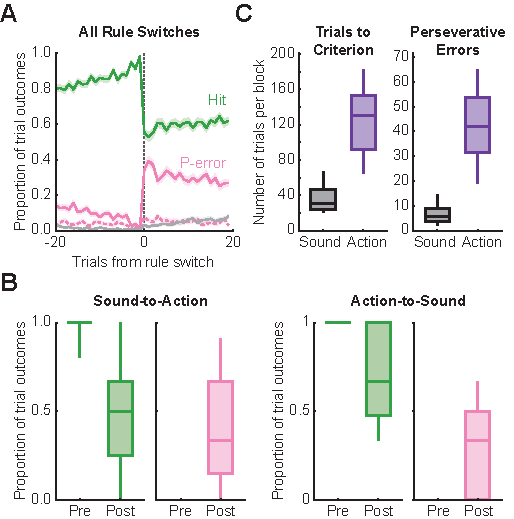
\includegraphics[width=8.7cm]{Figures/Chapter4/Fig3} 
\end{center}

\caption[Formal measures of task performance]
{Formal measures of task performance. (A) Mean proportion of hits (green), perseverative errors (solid pink), other errors (dashed pink), and misses (gray) as a function of the number of trials from a rule switch across all sessions ($N=64$). Shading, SEM. (B) Box plots representing the mean proportion of hits (green) and preseverative errors (pink) for trials immediately preceding a rule switch (Pre) and for trials immediately following one (Post). Results are presented separately for switches from the sound rule to an action rule (left), and vice-versa (right). (C) Box plots representing the number of trials taken to reach criterion (left), and the number of perseverative errors committed (right), during sound (black) and action blocks (purple). All boxes represent quartiles 1--3; whiskers represent 9th and 91st percentiles.}

\label{fig:Fig3}
\end{figure}

As expected, accuracy dropped precipitously following a rule switch (\ref{fig:Fig3}A). The proportion of hits decreased from $98 \pm 1 \%$ in the trial before a rule switch, to $55 \pm 2 \%$ in the next trial (paired $t_{63} =16.8$, $p=\num{5e-25}$). This reduction in accuracy was mostly attributable to an increase in perseverative errors, which accounted for $0 \pm 0 \%$ of trials immediately preceding a rule switch and $35 \pm 2 \%$ of trials immediately following (paired $t_{63}=14.0$, $p=\num{4e-21}$). A much smaller increase was noted in the proportion of other errors ($\Delta=6\%$, paired $t_{63}=3.8$, $p=\num{3e-4}$) and misses ($\Delta=3\%$, paired $t_{63}=3.6$, $p=\num{7e-4}$). 

Results of this analysis are presented separately for switches from the sound rule to an action rule, and vice-versa, in Figure \ref{fig:Fig3}B. In both cases, the proportion of hits decreased substantially in the trial following a rule switch (sound-to-action: $\Delta=51\%$, paired $t_{63} =12.4$, $p=\num{1e-18}$; action-to-sound: $\Delta=35\%$, paired $t_{63} =8.8$, $p=\num{2e-12}$). Following a sound-to-action rule switch, the proportion of hits was indistinguishable from chance, at $46 \pm 4 \%$ ($t_{63}=1.0$, $p=0.30$; one-sample t-test for the null hypothesis, $H_0:\Delta=0.5$). In the case of action-to-sound rule switches, it remained significantly greater than chance, at $65 \pm 4 \%$ (one-sample $t_{63}=3.9$, $p=\num{2e-4}$). In both cases, the proportion of perseverative errors increased significantly (sound-to-action: $\Delta=39\%$, paired $t_{63} =10.1$, $p=\num{1e-14}$; action-to-sound: $\Delta=29\%$, paired $t_{63} =8.6$, $p=\num{3e-12}$).  

Although subjects were capable of adjusting sensorimotor decisions to both rule types, in general, they adapted more readily during action-to-sound rule transitions than the reverse (Fig. \ref{fig:Fig3}C). Substantially fewer trials were taken to reach the accuracy criterion in sound as compared to action blocks ($39 \pm 3$ vs. $126 \pm 6$; paired $t_{63} =13.2$, $p=\num{9e-20}$), and fewer perseverative errors were committed before the criterion was reached ($7 \pm 1$ vs. $43 \pm 2$; paired $t_{63} =14.0$, $p=\num{5e-21}$).

\nnsub{Task-Related Modulation of Neural Activity}

To gain insight into how distinct cell types in MFC contribute to the encoding of task-relevant information, we examined the recruitment patterns of GCaMP\textsuperscript{+} SST, VIP, PV, and PYR neurons both within and across trials. Example fields-of-view, along with cellular fluorescence time series obtained from each cell type, are shown in Figure \ref{fig:Fig4}A--H. 

\begin{figure}[htbp]

\begin{center}
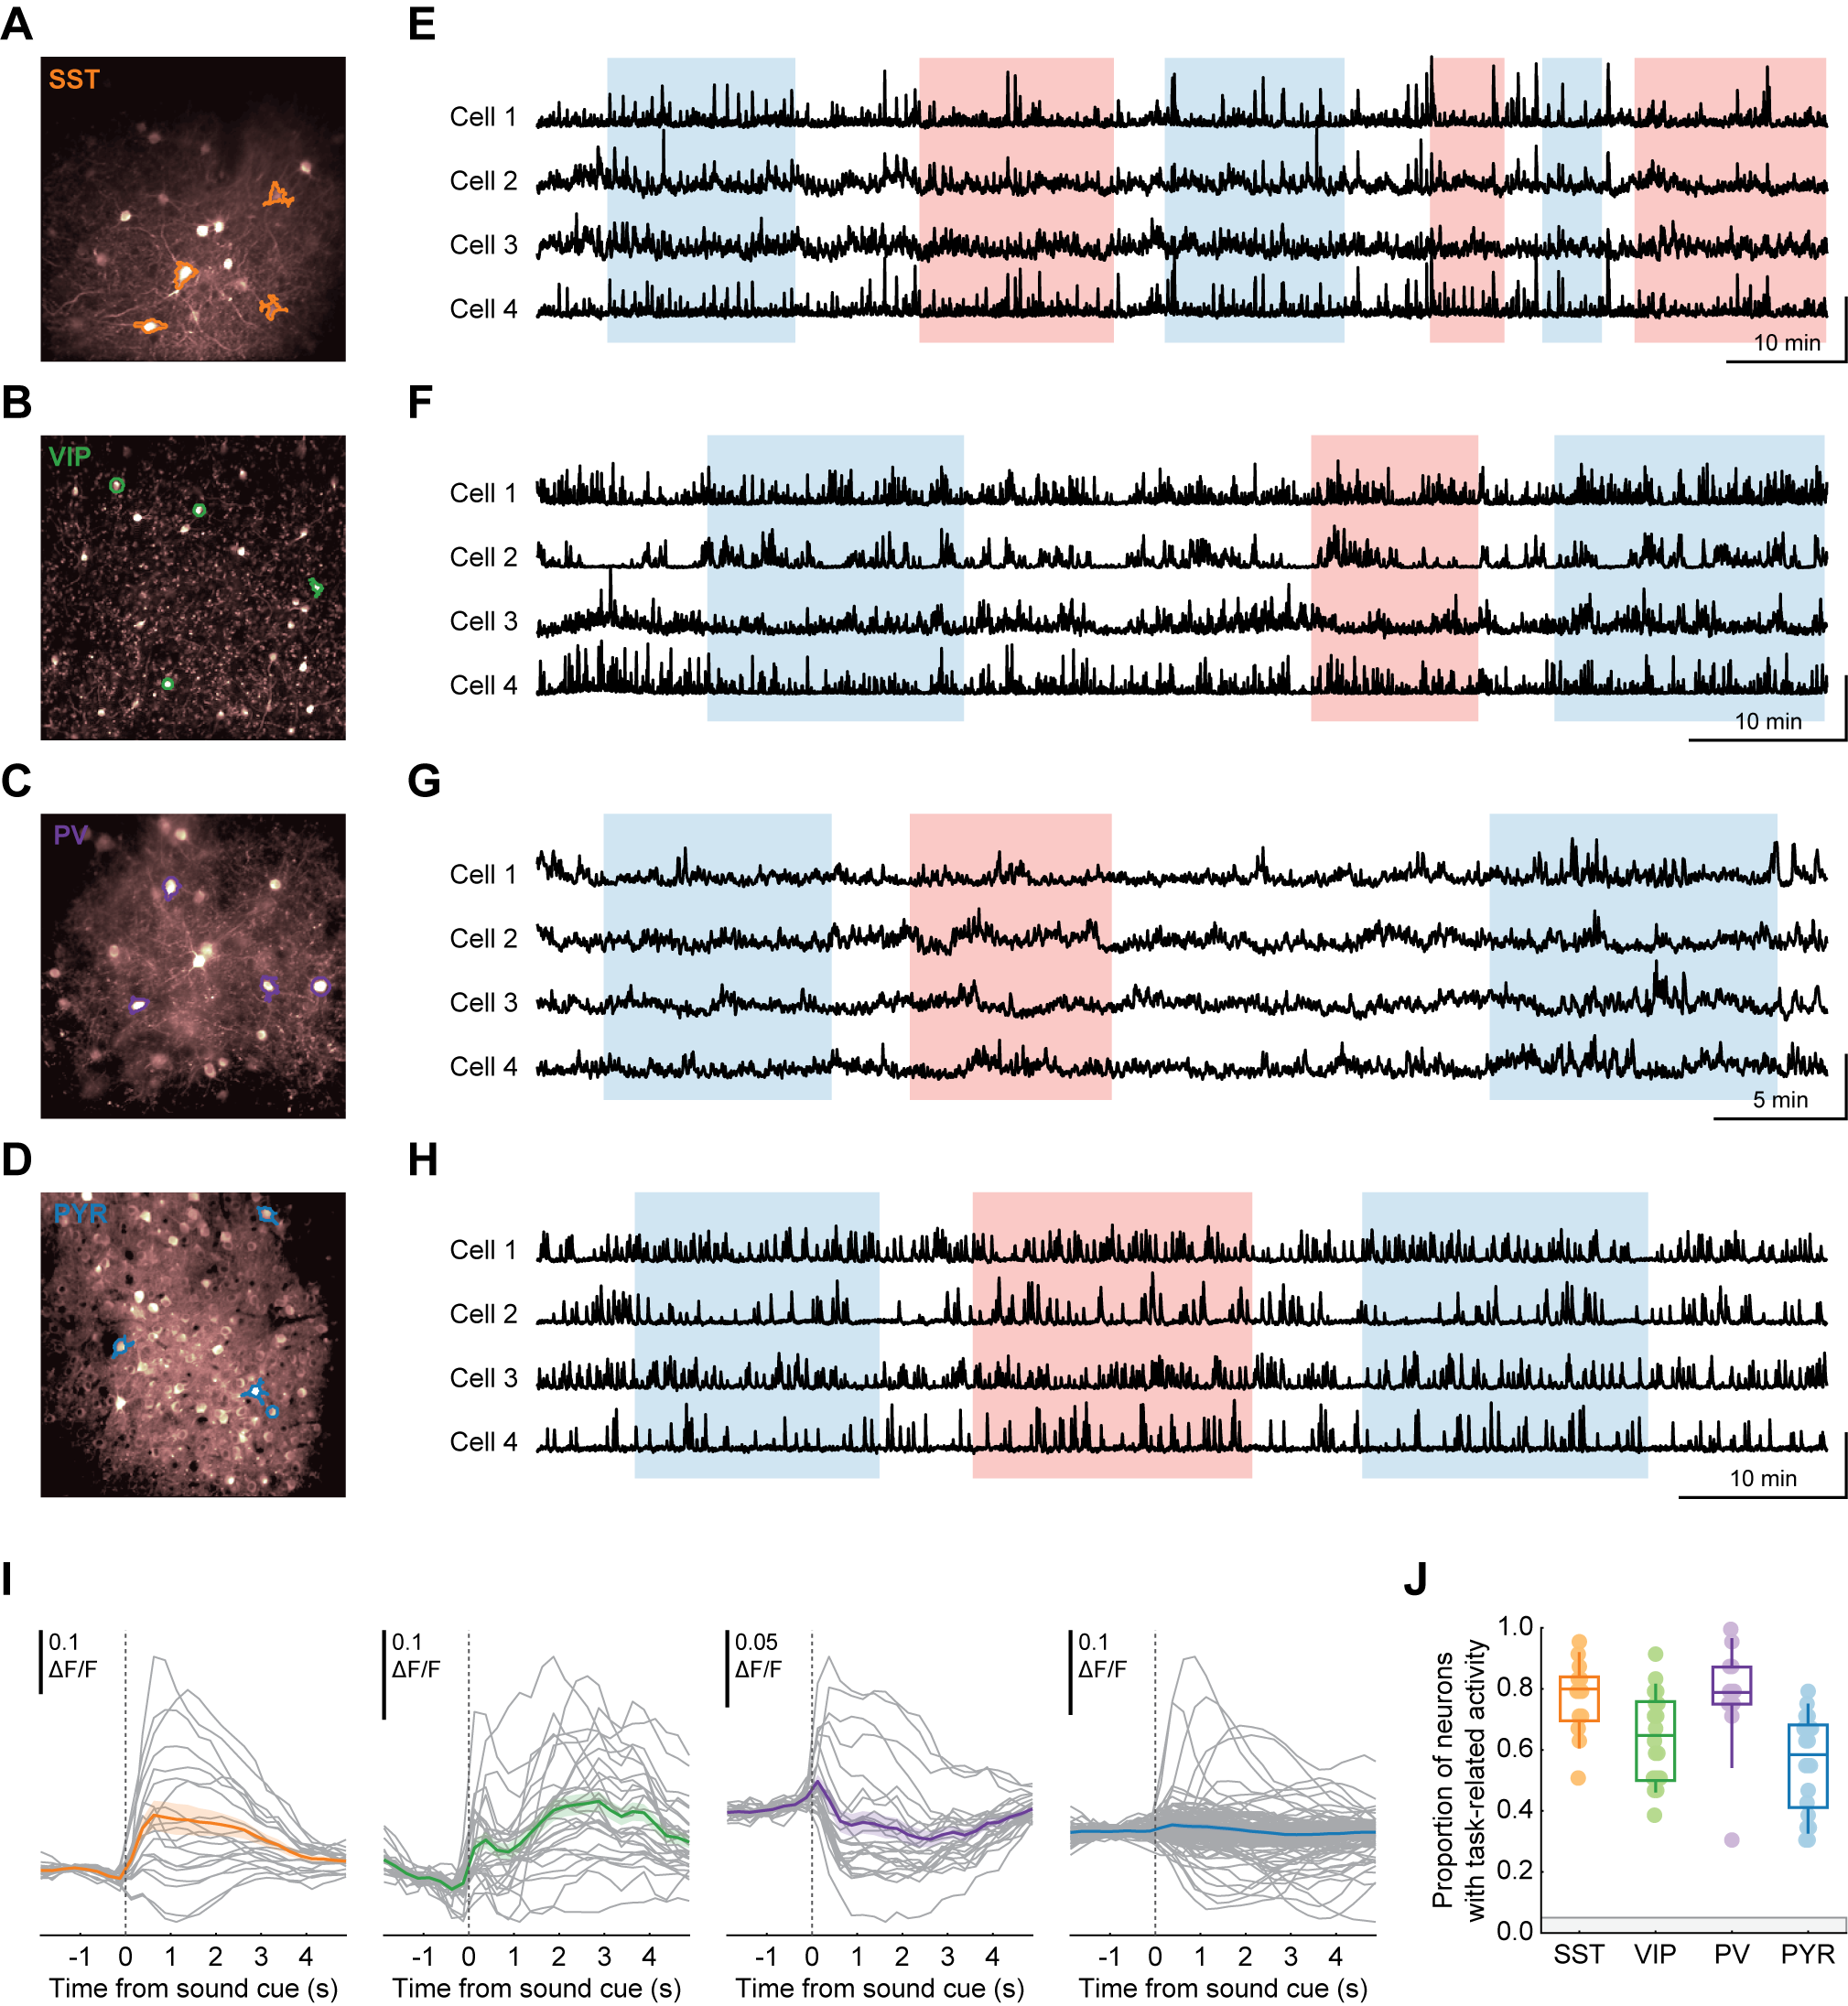
\includegraphics[width=\textwidth]{Figures/Chapter4/Fig4} 
\end{center}

\caption[Task-related neural activity in SST, VIP, PV, and PYR neurons]
{Task-related neural activity in SST, VIP, PV, and PYR neurons. (A--D) Mean projections from example fields-of-view showing SST, VIP, PV, and PYR neurons, respectively. (E--H) Example $\frac{\Delta F}{F}$ traces from the sessions in A--D. Red and blue background shading correspond to the action-left and action-right rule, respectively. White background indicates periods governed by the sound rule. Vertical scale bar, 1 SD (I) Mean $\frac{\Delta F}{F}$ traces from the sessions shown in E--H, presented as a function of time relative to the sound cue. Grey lines represent the mean trace for each neuron across all completed trials, re-centered on the mean value obtained during the pre-cue period. The grand $\mathit{mean} \pm \mathit{SEM}$ across all cells is overlaid in color. (J) Proportion of task-modulated neurons within each cell type, across $N=$ 13, 19, 12, and 20 sessions from SST, VIP, PV, and PYR neurons, respectively.}

\label{fig:Fig4}
\end{figure}

All cellular fluorescence data are presented as $\frac{\Delta F}{F}$, which was calculated for each time point as $(F(t)-F_0(t))/F_0(t)$, where $F(t)$ is the mean of the raw fluorescence measured from the cell body at time $t$, and $F_0(t)$ is the 5th percentile of $F$ across a 10 min sliding window centered at time $t$. We focused on $\frac{\Delta F}{F}$ traces spanning the period from -2 to 5 s relative to each sound cue to examine time-dependent activity changes within each trial (Fig. \ref{fig:Fig4}I--J), and across trials that differed with respect to choice, outcome, and the current rule (Figs. \ref{fig:Fig5}--\ref{fig:Fig8}).

We quantified the sensitivity of SST, VIP, PV, and PYR populations to the temporal structure of the task by comparing the mean $\frac{\Delta F}{F}$ measured in the 2 s preceding each sound cue with that of the 5 s following it. Neurons showing a significant difference across these two epochs ($p<0.05$, Wilcoxon signed-rank test) were considered to have been modulated by the task. These included $78 \pm 5\%$ of PV, $77 \pm 3\%$ of SST, $63 \pm 3\%$ of VIP, and $56 \pm 4\%$ of PYR neurons (Fig. \ref{fig:Fig4}J). 

The proportion of task-modulated neurons varied significantly across cell types (Kruskal-Wallis $H_{3,60}=21.5$, $p=\num{8e-5}$). In particular, PYR populations included a significantly smaller proportion than either PV ($p=\num{9e-4}$, Tukey test) SST populations ($p=\num{1e-3}$, Tukey test). Tukey's post hoc test revealed no significant difference between PYR and VIP populations in this regard ($p=0.61$). PV and SST populations were likewise statistically indistinguishable ($p=1$). 

These results indicate task-related activity in substantial fractions of all four cell types. However, the activities of PV and SST neurons were preferentially modulated.

\nnsub{Modulation by Specific Task Variables}

Next, we examined the capacity of each cell type to encode specific behavioral variables crucial for task performance---namely, choices, outcomes, and rules. As an estimate for signal reliability in individual neurons, we calculated a modulation index based on the receiver operating characteristic (ROC) given by the responses of each neuron in varied trial conditions \citep{barlow1971responses,feierstein2006representation}. 

In the context of signal detection, the ROC captures the trade-off between sensitivity and specificity as detection parameters are varied. This relationship can be estimated empirically by taking the true positive rate (TPR) as a function of the false positive rate (FPR) at a series of detection thresholds. 

The area under the resulting curve (AUC) may serve as an unbiased scalar metric for signal discriminability. For example, if the neural activity levels associated with rewarded versus unrewarded trials yielded an AUC approaching 0 or 1, then an ideal observer could predict the trial outcome with an accuracy close to 100\% using these physiological data alone. By contrast, at an AUC of 0.5, chance-level accuracy would be expected. 

To assess choice, outcome, and rule signaling in each neuron, we calculated a modulation index $I(t) = 2(\mathit{AUC} - 0.5)$ as a function of time relative to the start of each trial, using cellular fluorescence traces obtained during subsets of trials that differed according to the behavioral variable of interest. For each variable, one subset of trials was arbitrarily chosen as the positive class ($\mathit{choice}=\mathit{left}$, $\mathit{outcome}=\mathit{reward}$, or $\mathit{rule}=\mathit{sound}$), and the remaining subset was assigned to the negative class ($\mathit{choice}=\mathit{right}$, $\mathit{outcome}=$ \emph{no reward}, or $\mathit{rule}=\mathit{action}$). Thus, $I(t)$ could range from -1 to 1, with positive and negative values reflecting a preference for positive and negative trials, respectively, and its magnitude $M(t)$ reflecting the signal reliability irrespective of preference.

\begin{figure}[htbp]

\begin{center}
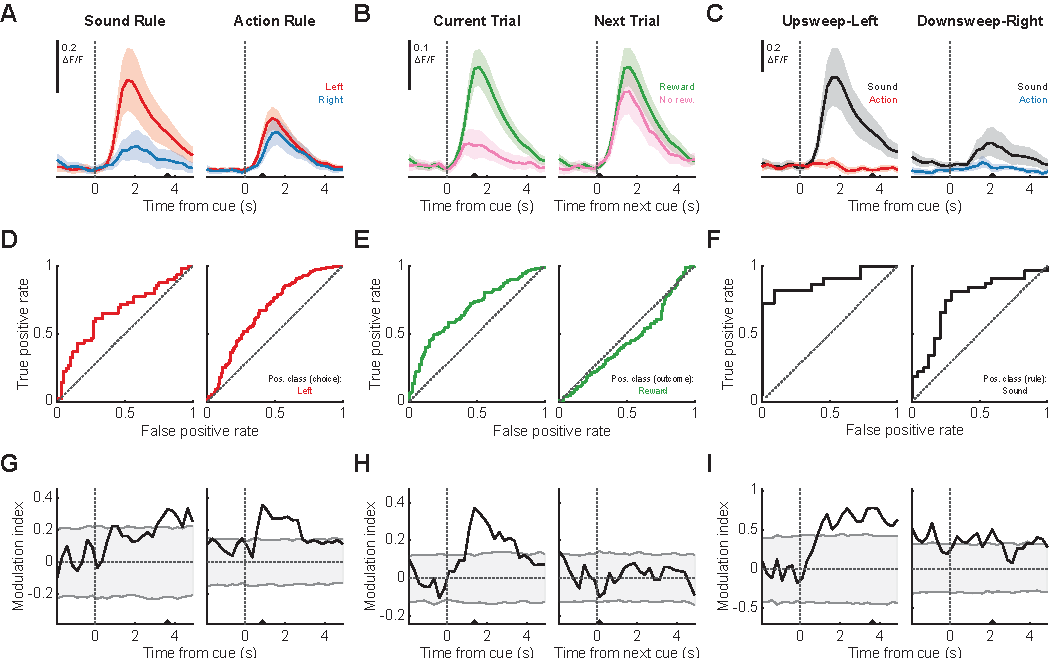
\includegraphics[width=\textwidth]{Figures/Chapter4/Fig5}
\end{center}

\caption[Example cell modulated by choice, outcome, and rule context]
{Example cell modulated by choice, outcome, and rule context. (A) Mean $\frac{\Delta F}{F}$ traces from a single PYR neuron as a function of time relative to cue onset. Traces were averaged across trials in which the left (red) or right (blue) spout was chosen. Results are presented separately for trials governed by the sound (left) and action rule (right). Shading, bootstrapped 95\% confidence intervals. (B) Mean traces associated with rewarded (green) or unrewarded choices (pink) made in the current trial. Results are plotted as a function of time relative to cue onset in the current trial (left) and the trial immediately following the indicated outcome (right). (C) Mean traces from sound vs. action trials in which the same choice was made in response to the same sound cue and resulted in a reward. Left: upsweep-left trials governed by the sound (black) or action-left rule (red). Right: downsweep-right trials governed by the sound (black) or action-right rule (blue). (D--F) Example ROC curves calculated at the time points indicated by black arrowheads in A--C. Left trials, rewarded trials, and sound trials were arbitrarily assigned positive class membership for the analysis of choice, outcome, and rule signals, respectively. (G--I) The modulation index $I$, plotted as a function of time relative to cue onset for the full series of time points in A--C. For each time $t$, $I(t)$ was calculated from the area under the corresponding ROC curve (AUC) as $2*(\mathit{AUC}-0.5)$. The shaded intervals reflect the middle 95\% of $I_{0}(t)$, a null distribution generated by replicating the analysis using shuffled class labels.}

\label{fig:Fig5}
\end{figure}

As a summary for signal reliability within each cell type, we took two scalar estimates for each session: the mean modulation magnitude $\Bar{M}$, and the proportion of significantly modulated neurons $P$. $\Bar{M}$ was calculated as the grand mean of the modulation magnitude across all neurons during the first 5 s of the trial. $P$ was the proportion of neurons in which ${M}$ rose above chance for $\ge 1$ s within the same period. For example, Figure \ref{fig:Fig5} shows a PYR neuron that was significantly modulated by choice, outcome, and rule.

To summarize preference, we calculated the mean modulation index $\Bar{I}$ across neurons in each session, as well as the proportion of neurons with a significant preference for positive and negative trials (eg, $P_{\mathit{left}}$ and $P_{\mathit{right}}$). 

A Wilcoxon signed-rank test was used to compare $\Bar{M}$ or $\Bar{I}$ across sessions with the corresponding null results, and to compare $P$ with a corresponding set of false discovery rate estimates (FDR; see \hyperlink{methods_ROC}{Methods}). 

\nnsubsub{Choice-Related Modulation}

To examine choice-related modulation, we grouped $\frac{\Delta F}{F}$ traces according to whether the left or right spout was chosen in the corresponding trial. Sound and action trials were considered separately, and the analysis was limited to rewarded choices. 

The activity of all four cell types was modulated by choices made during the sound rule. In each case, modulation magnitude ${M}_{choice}(t)$ rose to significance within 250 ms of cue onset (Fig. \ref{fig:Fig6}A). The mean modulation magnitude $\Bar{M}_{\mathit{choice}}$ was significant for all four cell types, both in the current trial (SST: $\Bar{M}=0.14\pm0.01$, $W_{13}=1$, $p=\num{4e-4}$; VIP: $\Bar{M}=0.12\pm0.01$, $W_{19}=0$, $p=\num{1e-4}$; PV: $\Bar{M}=0.12\pm0.01$, $W_{12}=2$, $p=\num{0.001}$; PYR: $\Bar{M}=0.13\pm0.01$, $W_{20}=1$, $p=\num{1e-4}$), and the following trial (SST: $\Bar{M}=0.11\pm0.01$, $W_{13}=10$, $p=\num{0.01}$; VIP: $\Bar{M}=0.10\pm0.01$, $W_{19}=44$, $p=\num{0.04}$; PV: $\Bar{M}=0.10\pm0.01$, $W_{12}=9$, $p=\num{0.02}$; PYR: $\Bar{M}=0.11\pm0.01$, $W_{20}=46$, $p=\num{0.03}$).

\begin{figure}[htbp]

\begin{center}
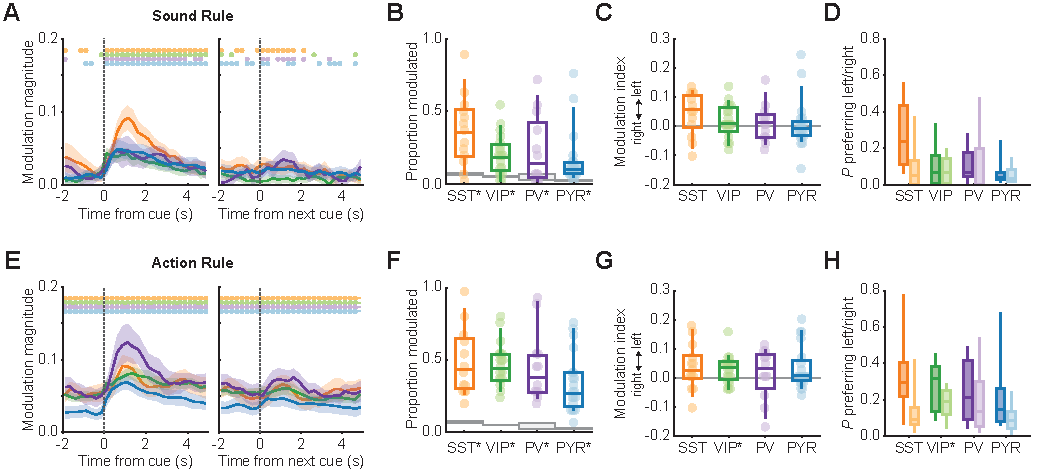
\includegraphics[width=\textwidth]{Figures/Chapter4/Fig6}
\end{center}

\caption[Choice-related modulation]
{Choice-related modulation. (A) Modulation magnitude $M$ with respect to the choice made in the current trial, plotted as a function of time relative to cue onset in the current trial (left) and the next trial (right). $M_{\mathit{choice}}(t)$ is presented as the difference from a null distribution obtained when the same analysis was conducted using shuffled choices. Line plots with shaded confidence intervals represent the $\mathit{mean} \pm \mathit{SEM}$ within SST (orange), VIP (green), PV (purple), and PYR populations (blue). Solid circles above indicate time bins where the corresponding cell type differed significantly from chance ($p<0.05$, Wilcoxon signed-rank test vs. shuffle). (B) The proportion of each cell population $P_{\mathit{choice}}$ that exhibited significant choice-related modulation in the current trial. (C) The mean modulation index $\bar{I}_{\mathit{choice}}$, calculated from the first 5 s of the current trial. (D) The proportion of each cell population exhibiting a significant preference for left ($P^+$) and right choices ($P^-)$, represented respectively in paired box plots to the left and right. (E--H) Same as A--C, for action blocks. For B--D and F--H, boxes indicate quartiles 1--3 and whiskers indicate the 9th and 91st percentiles of the empirical distribution. Values from individual sessions are represented in the beeswarm plots. Grey boxes represent quartiles 1 and 3 of the null distribution (visually indistinguishable from zero in C and G). Asterisks in B--C and F--G indicate significant differences from the null distribution for each cell type; in D and H, they indicate significant differences between $P^+$ and $P^-$ within each cell type; both were assessed at $\alpha = 0.05$, Wilcoxon signed-rank test. $N=$ 13 SST, 19 VIP, 12 PV, and 20 PYR populations.}

\label{fig:Fig6}
\end{figure}

Significant proportions of SST ($37\pm7\%$, $W_{13}=2$, $p=\num{7e-4}$), VIP ($20\pm3\%$, $W_{19}=7$, $p=\num{4e-4}$), PV ($23\pm7\%$, $W_{12}=6$, $p=\num{0.007}$), and PYR neurons ($17\pm4\%$, $W_{20}=0$, $p=\num{9e-5}$) were differentially recruited based on choice ($P_{\mathit{choice}}$; Fig. \ref{fig:Fig6}B). No significant differences in either $\Bar{M}_{\mathit{choice}}$ (Kruskal-Wallis $H_{3,60}=5.5$, $p=0.14$) or $P_{\mathit{choice}}$ ($H_{3,60}=5.6$, $p=0.16$) were found among cell types during the sound rule.

No substantial preference for left or right choices was evident at the population level for any of the cell types examined. In each case, the mean modulation index $\Bar{I}_{\mathit{choice}}$ did not differ significantly from chance ($p>0.05$ vs. shuffle; Fig. \ref{fig:Fig6}C). Moreover, the proportions of neurons exhibiting significant preference for left and right choices were approximately balanced within the VIP ($11\pm3\%$ vs. $9\pm2\%$, $W_{17}=66$, $p=0.62$), PV ($11\pm3\%$ vs. $12\pm6\%$, $W_{10}=25$, $p=0.85$), and PYR populations ($8\pm3\%$ vs. $8\pm3\%$, $W_{19}=88$, $p=0.78$) (Fig. \ref{fig:Fig6}D). Left-preferring neurons appeared to predominate within the SST population (left: $27\pm6\%$ vs. right: $10\pm4\%$), but the difference fell short of significance ($W_{12}=14.5$, $p=0.06$).

\paragraph{}
During the action rule, choices were reflected for the entirety of the trial in the activity of all four cell types. In each case, the modulation magnitude $M_{\mathit{choice}}(t)$ was significant throughout the 2 s leading up to the sound cue, and remained above chance in the 2 s before the next cue ($p>0.05$ vs. shuffle; Fig. \ref{fig:Fig6}E).\footnote{One limitation of our analysis is that the action rule reinforces repetition of a rewarded choice, leading to increased correlation between consecutive choices. Interpretation of $M_{\mathit{choice}}$ in this case remains somewhat ambiguous because the observed signals may reflect a combination of choice history and the current choice. For this reason, we only examined $\Bar{M}_{\mathit{choice}}$ in the current trial.} 

Accordingly, the mean modulation magnitude during action trials was significant for all cell types (SST: $\Bar{M}=0.14\pm0.01$, $W_{13}=0$, $p=\num{2e-4}$; VIP: $\Bar{M}=0.14\pm0.01$, $W_{19}=0$, $p=\num{1e-4}$; PV: $\Bar{M}=0.16\pm0.02$, $W_{12}=0$, $p=\num{5e-4}$; PYR: $\Bar{M}=0.11\pm0.01$, $W_{20}=0$, $p=\num{9e-5}$). A Kruskal-Wallis test revealed significant differences in $\Bar{M}_{\mathit{choice}}$ across cell types ($H_{3,60}=7.9$, $p=0.048$). However, no individual comparisons were significant (all $p>0.05$, Tukey test). 

Substantial proportions of all cell types were differentially recruited based on the choices made during action trials (SST: $48\pm7\%$, $W_{13}=0$, $p=\num{2e-4}$; VIP: $46\pm3\%$, $W_{19}=0$, $p=\num{1e-4}$; PV: $45\pm7\%$, $W_{12}=0$, $p=\num{5e-4}$; PYR: $34\pm5\%$, $W_{20}=0$, $p=\num{9e-5}$; Fig. \ref{fig:Fig6}F). No significant differences in $P_{\mathit{choice}}$ were found among cell types (Kruskal-Wallis $H_{3,60}=5.0$, $p=0.17$).

A significant overall preference for left or right choices was observed only among VIP neurons, which were preferentially active during trials where the left (contralateral) spout was chosen. The mean modulation index within VIP populations was significantly positive ($\Bar{I}=0.04\pm0.01$, $W_{19}=31$, $p=\num{0.01}$; Fig. \ref{fig:Fig6}G), and they contained a greater proportion of left- as compared to right-preferring neurons ($28\pm3\%$ vs. $18\pm2\%$, $W_{18}=40$, $p=0.048$; Fig. \ref{fig:Fig6}H). However, trends toward a contralateral population preference were also noted in SST ($P_{\mathit{left}}$: $34\pm7\%$ vs. $14\pm4\%$, $W_{11}=13$, $p=0.08$) and PYR populations ($24\pm5\%$ vs. $10\pm2\%$, $W_{20}=55$, $p=0.06$). No significant differences in $\Bar{I}$ were found between cell types (Kruskal-Wallis $H_{3,60}=0.4$, $p=0.95$). 

Comparisons of choice-related modulation across rule contexts revealed significantly stronger choice signals during action trials than during sound trials in all cell populations except SST. The difference was evident in both mean modulation magnitude (SST: $W_{13}=27$, $p=\num{0.22}$; VIP: $W_{19}=5$, $p=\num{3e-4}$; PV: $W_{12}=0$, $p=\num{5e-4}$; PYR: $W_{20}=23$, $p=\num{2e-3}$) and the proportion of each population exhibiting significant modulation (SST: $W_{13}=25$, $p=\num{0.17}$; VIP: $W_{19}=0$, $p=\num{1e-4}$; PV: $W_{12}=2$, $p=\num{1e-3}$; PYR: $W_{20}=18$, $p=\num{1e-3}$). 

Taken together, these results implicate all cell types examined in the representation of choices in M2. Choice signaling was evident during the current trial regardless of which rule was being enforced, but was more pronounced during the action rule. The summation of signals related to current and prior choices may partially account for this difference, due to the repetition of choices demanded by the action rule. During the sound rule, sustained choice-related activity was clearly evident in all four cell types, and persisted subsequent to the next sound cue. We also found limited evidence for preferential activity surrounding contralateral choices during action but not sound blocks---a trend that rose to significance only in VIP populations.       

\nnsubsub{Outcome-Related Modulation}
To investigate outcome-related modulation, we considered traces associated with rewarded vs. unrewarded choices, ie, hits vs. errors. We separately examined effects of the current trial outcome on neural activity in the current and subsequent trial. For the current trial, the previous outcome was held constant by limiting the analysis to $\frac{\Delta F}{F}$ traces preceded by a rewarded choice. Likewise, for the subsequent trial we held the corresponding outcome constant by focusing on traces associated with rewarded choices.

All cell types exhibited differential activity based on the trial outcome. Across cell types, modulation magnitude $M_{\mathit{outcome}}(t)$ was significant for all time bins $\ge 250$ ms following the sound cue, and the associated signals persisted well into the next trial ($p<0.05$, Wilcoxon signed-rank test; Fig. \ref{fig:Fig7}A). 
% \begin{SCfigure}[][htbp]
\begin{figure}[htp]

\begin{center}
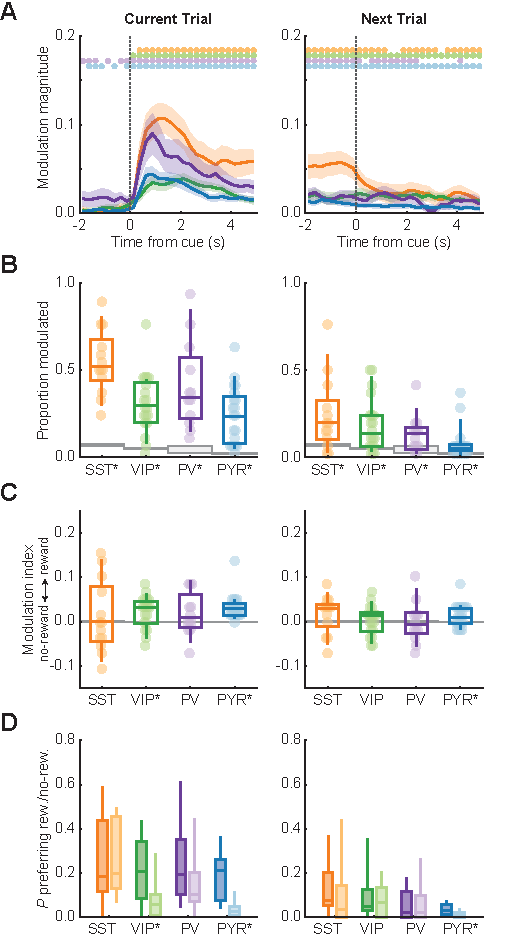
\includegraphics[width=8.7cm]{Figures/Chapter4/Fig7}
\end{center}

\caption[Outcome-related modulation]
{Outcome-related modulation. (A) Modulation magnitude $M$ with respect to the outcome of the current (left) and prior trial (right), plotted as in Figure \ref{fig:Fig6}A. Solid circles indicate time bins where $M_{\mathit{outcome}}(t)$ differed significantly from chance ($p<0.05$, Wilcoxon signed-rank test vs. shuffle) within SST (orange), VIP (green), PV (purple), and PYR populations (blue). (B) The proportion of each cell population, $P_{\mathit{outcome}}$, that exhibited significant modulation associated with the current (left) or prior outcome (right). (C) The mean modulation index $\bar{I}_{\mathit{outcome}}$ associated with the current (left) and prior outcome (right), calculated from the first 5 s of the trial. (D) The proportion of each cell population exhibiting a significant preference for rewarded ($P^+$; dark shading) and unrewarded choices ($P^-$; light shading), represented respectively in paired box plots. Left and right axes present the results with respect to the current and prior outcome, respectively. Asterisks in B--C indicate significant differences from the null distribution for each cell type; in D, they indicate significant differences between $P^+$ and $P^-$ within each cell type; both were assessed at $\alpha = 0.05$, Wilcoxon signed-rank test. $N=$ 13 SST, 19 VIP, 12 PV, and 20 PYR populations. All plots presented as in Figure \ref{fig:Fig6}.}

\label{fig:Fig7}
% \end{SCfigure}
\end{figure}

% {Outcome-related modulation. (A) Modulation magnitude $M$ with respect to the outcome of the current (left) and prior trial (right), plotted as a function of time relative to the sound cue. $M_{\mathit{outcome}}(t)$ is presented as the difference from a null distribution obtained when the same analysis was conducted using shuffled choices. Line plots with shaded confidence intervals represent the $\mathit{mean} \pm \mathit{SEM}$ within SST (orange), VIP (green), PV (purple), and PYR populations (blue). Solid circles above indicate time bins where $M_{\mathit{outcome}}(t)$ differed significantly from chance ($p<0.05$, Wilcoxon signed-rank test). (B) The proportion of each cell population, $P_{\mathit{outcome}}$, that exhibited significant modulation associated with the current (left) or prior outcome (right). (C) The mean modulation index $\bar{I}_{\mathit{outcome}}$ associated with the current (left) and prior outcome (right), calculated from the first 5 s of the trial. (D) The proportion of each cell population exhibiting a significant preference for rewarded ($P^+$) or unrewarded choices ($P^-$), represented respectively in paired box plots. Left and right axes present the results with respect to the current and prior outcome, respectively. Asterisks in B--C indicate significant differences from the null distribution for each cell type; in D, they indicate significant differences between $P^+$ and $P^-$ within each cell type; both were assessed at $\alpha = 0.05$, Wilcoxon signed-rank test. All plots presented as in Figure \ref{fig:Fig5}.}

The mean modulation magnitude $\Bar{M}_{\mathit{outcome}}$ was significant in all four cell types across the current trial (SST: $\Bar{M}=0.13\pm0.01$, $W_{13}=0$, $p=\num{2e-4}$; VIP: $\Bar{M}=0.09\pm0.00$, $W_{19}=0$, $p=\num{1e-4}$; PV: $\Bar{M}=0.11\pm0.01$, $W_{12}=0$, $p=\num{5e-4}$; PYR: $\Bar{M}=0.08\pm0.01$, $W_{20}=0$, $p=\num{9e-5}$) as well as the following trial (SST: $\Bar{M}=0.08\pm0.01$, $W_{13}=4$, $p=\num{0.002}$; VIP: $\Bar{M}=0.08\pm0.00$, $W_{19}=0$, $p=\num{1e-4}$; PV: $\Bar{M}=0.07\pm0.01$, $W_{12}=10$, $p=\num{0.02}$; PYR: $\Bar{M}=0.06\pm0.00$, $W_{20}=13$, $p=\num{6e-4}$). 

In both cases, differences in $\Bar{M}_{\mathit{outcome}}$ among cell types were significant (current trial: Kruskal-Wallis $H_{3,60}=13$, $p=0.005$; next trial: $H_{3,60}=12$, $p=0.007$), with SST neurons showing the strongest modulation, and PYR neurons showing the weakest. During the current trial, SST neurons differed significantly from VIP ($p=0.03$, Tukey test) and PYR neurons ($p=0.006$). In the next trial, SST and VIP neurons both differed significantly from PYR neurons ($p=0.02$ for both comparisons). 
%  with respect to the outcome of current (Kruskal-Wallis $H_{3,60}=13$, $p=0.005$) as well as prior choices ($H_{3,60}=12$, $p=0.007$). 

Modulation by the outcome of the most recent choice persisted throughout the last 2 s of the intertrial interval in all cell types, but was most pronounced in SST neurons (Fig. \ref{fig:Fig7}A, right). During this period, the mean modulation magnitude $\Bar{M}_{\mathit{outcome}}$ differed significantly among cell types (Kruskal-Wallis $H_{3,60}=10.9$, $p=0.01$), and was significantly greater in SST ($\Bar{M}=0.11\pm0.01$) as compared to either VIP ($0.08\pm0.01$, $p=0.03$, Tukey test) or PYR neurons ($\Bar{M}=0.06\pm0.00$, $p=0.01$). The difference from PV neurons fell short of significance ($\Bar{M}=0.08\pm0.01$, $p=0.15$). 
% (SST: $\Bar{M}=0.11\pm0.01$; PV: $\Bar{M}=0.08\pm0.01$; VIP: $0.08\pm0.01$; PYR: $\Bar{M}=0.06\pm0.00$)

A similar pattern was evident in the proportion of neurons modulated by outcome $P_{\mathit{outcome}}$ (Fig. \ref{fig:Fig7}B). For all cell types, the proportion exceeded chance in both the current trial (SST: $55\pm5\%$, $W_{13}=0$, $p=\num{2e-4}$; VIP: $30\pm4\%$, $W_{19}=1$, $p=\num{2e-4}$; PV: $41\pm7\%$, $W_{12}=0$, $p=\num{5e-4}$; PYR: $24\pm4\%$, $W_{20}=0$, $p=\num{9e-5}$) and the next trial (SST: $24\pm6\%$, $W_{13}=6$, $p=\num{0.003}$; VIP: $19\pm3\%$, $W_{19}=15$, $p=\num{0.001}$; PV: $13\pm3\%$, $W_{12}=8$, $p=\num{0.01}$; PYR: $7\pm2\%$, $W_{20}=19$, $p=\num{0.001}$). In the current trial, $P_{\mathit{outcome}}$ differed significantly among cell types (Kruskal-Wallis $H_{3,60}=15$, $p=0.002$), and SST populations included a significantly greater proportion of outcome-modulated neurons than either VIP (Tukey test: $p=0.01$) or PYR populations ($p=0.002$). However, significant differences among cell types did not persist into the next trial ($H_{3,60}=5.8949$, $p=0.12$).

% $P_{\mathit{outcome}}$ differed among cell types (Kruskal-Wallis $H_{3,60}=15$, $p=0.002$), and individual comparisons revealed a pattern similar to $\Bar{M}_{\mathit{outcome}}$. Namely, the proportion was greatest in SST populations and smallest in PYR populations. SST populations included a significantly greater proportion of outcome-modulated neurons than either VIP (Tukey test: $p=0.01$) or PYR populations ($p=0.002$). However, significant differences in $P_{\mathit{outcome}}$ did not persist into the next trial ($H_{3,60}=5.8949$, $p=0.12$).

An overall preference for rewarded choices was observed among PYR and VIP neurons (Fig. \ref{fig:Fig7}C). For both cell types, the mean modulation index $\Bar{I}_{\mathit{outcome}}$ was significantly positive (PYR: $\Bar{M}=0.032\pm0.006$, $W_{20}=1$, $p=\num{1e-4}$; VIP: $\Bar{M}=0.021\pm0.008$, $W_{19}=38$, $p=\num{0.02}$). PYR neurons also maintained a significantly positive $\Bar{I}_{\mathit{outcome}}$ into the next trial ($\Bar{M}=0.014\pm0.006$, $W_{20}=49$, $p=\num{0.04}$).

Furthermore, the proportion of neurons with preferential activity during rewarded trials outnumbered those preferring the absence of reward in both PYR ($20\pm3\%$ vs. $4\pm1\%$, $W_{20}=1$, $p=\num{1e-4}$) and VIP populations ($22\pm3\%$ vs. $9\pm2\%$, $W_{17}=28$, $p=\num{0.02}$; Fig. \ref{fig:Fig7}D). The proportions were approximately balanced within SST populations ($27\pm6\%$ vs. $28\pm5\%$, $W_{12}=39$, $p=\num{1}$), and did not differ significantly in PV populations ($25\pm6\%$ vs. $16\pm5\%$, $W_{11}=22$, $p=\num{0.37}$). In PYR populations, reward-preferring neurons continued to predominate into the next trial, although both proportions were greatly diminished ($5\pm2\%$ vs. $2\pm1\%$, $W_{17}=33.5$, $p=\num{0.04}$).

A Kruskal-Wallis test revealed no significant differences in $\Bar{I}_{\mathit{outcome}}$ among cell types, either in the current ($H_{3,60}=2.5$, $p=0.47$) or following trial ($H_{3,60}=3.3$, $p=0.34$). 

Collectively, these results indicate that trial outcomes were represented in the activity of all four cell types examined. Signals reflecting the outcome of the current choice rose to significance within 500 ms of the sound cue, consistent with the mean response time of $208 \pm 5$ ms in this set of experiments (IQR: 172--225 ms). In all cell types, the outcome signal persisted throughout the current trial, and well into the subsequent trial. SST activity exhibited the strongest modulation, with signals remaining notably elevated throughout the intertrial interval. Interestingly, SST populations contained roughly balanced proportions of neurons with preferential activity following rewarded and unrewarded choices, whereas PYR and VIP populations were more heavily recruited by reward.

\nnsubsub{Context-Related Modulation}
Finally, we examined modulation based on the rule context governing reinforcement in the current trial. For parity between sound and action trials, we only compared traces from trials where the same choice was made in response to the same sound cue (eg, upsweep-left-sound and upsweep-left-action trials). Additionally, we limited the analysis to rewarded choices made during the final twenty trials of each block---the period when choices were most consistent with the current rule.

Context-related modulation was observed in all cell types throughout the duration of the trial. In each case, $M_{\mathit{rule}}(t)$ was significant for all time bins during upsweep-left trials ($p<0.05$, Wilcoxon signed-rank test), and with the exception of SST neurons ($p<0.05$ in 15/20 bins), was also significant for all time bins during downsweep-right trials (Fig. \ref{fig:Fig8}A). In VIP, PV, and PYR neurons, $M_{\mathit{rule}}(t)$ was also significant for all time bins prior to the sound cue. SST neurons exhibited significant modulation throughout this period only during upsweep-left trials.

\begin{figure}[htbp]

\begin{center}
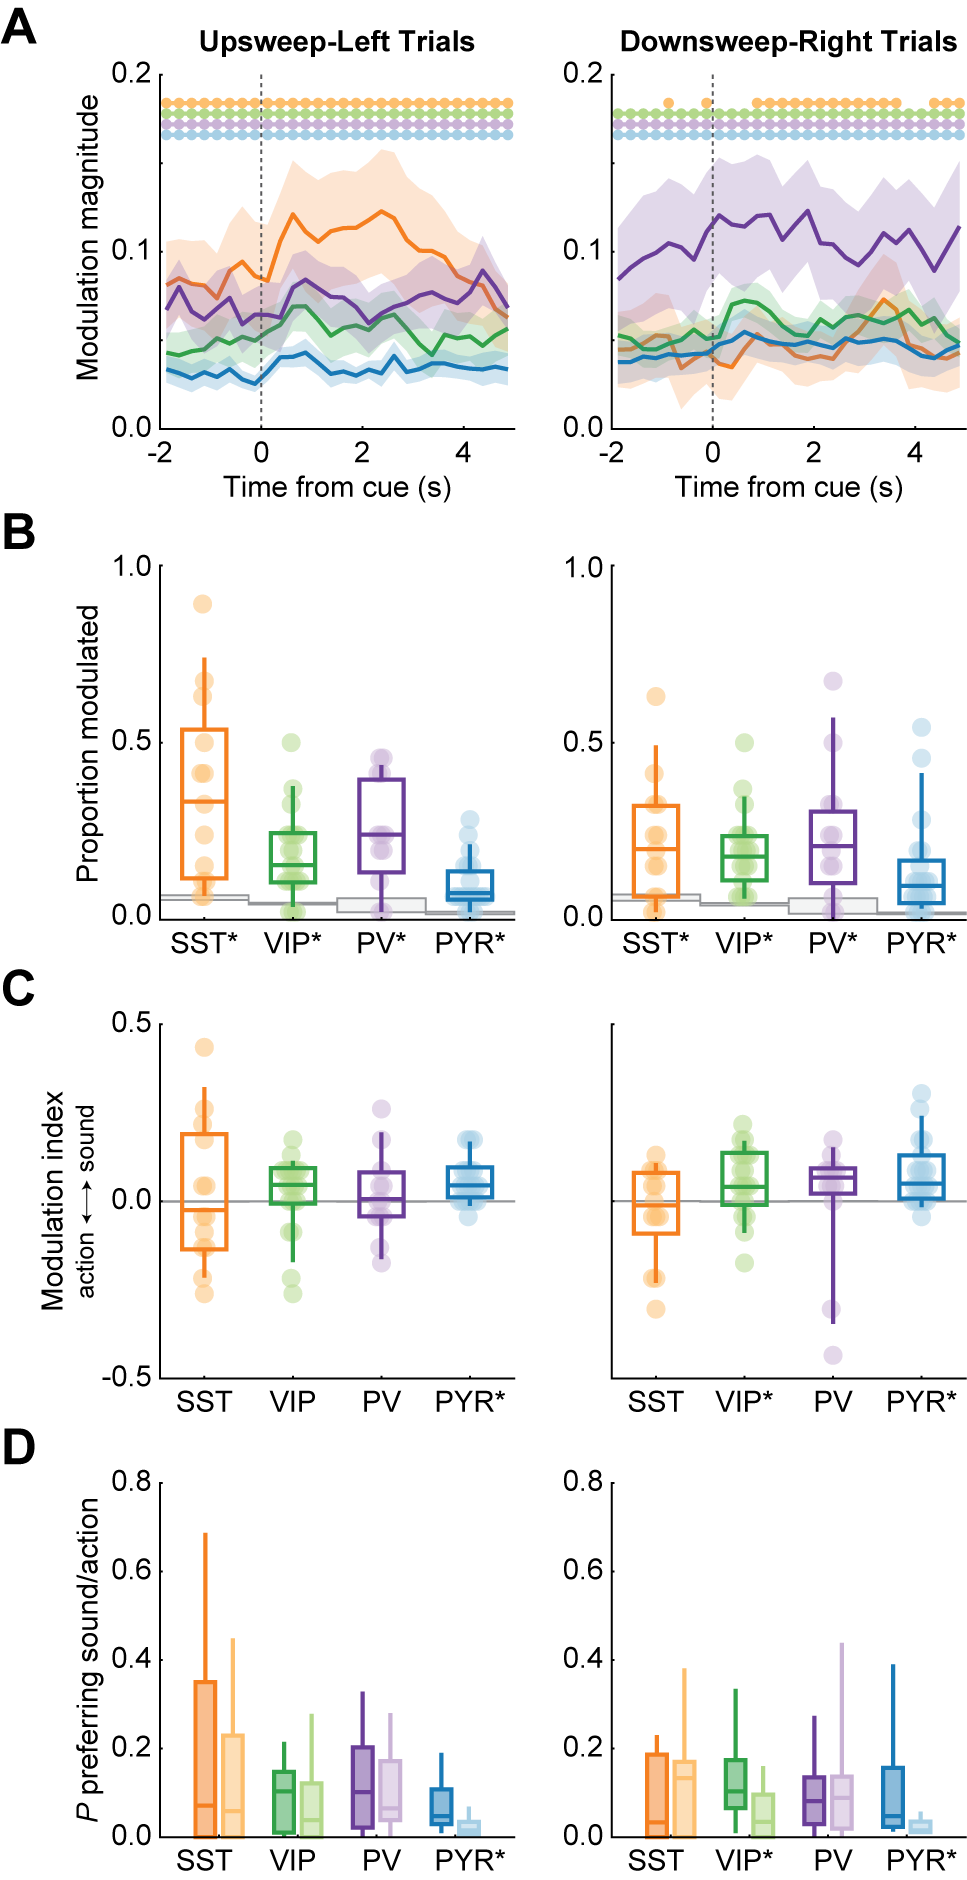
\includegraphics[width=8.7cm]{Figures/Chapter4/Fig8} 
\end{center}

\caption[Context-related modulation]
{Context-related modulation. Modulation by the current rule was examined under matched trial conditions: upsweep trials in which a left choice was rewarded (left), and downsweep trials in which a right choice was rewarded (right). (A) Modulation magnitude $M_{\mathit{rule}}(t)$ with respect to the rule governing the current trial (sound vs. action), plotted as in Figure \ref{fig:Fig6}A. Solid circles indicate time bins where $M_{\mathit{rule}}(t)$ differed significantly from chance ($p<0.05$, Wilcoxon signed-rank test vs. shuffle) within SST (orange), VIP (green), PV (purple), and PYR populations (blue). (B) The proportion of each cell population, $P_{\mathit{rule}}$, that exhibited significant modulation associated with the current rule. (C) The mean modulation index $\bar{I}_{\mathit{rule}}$, calculated from the first 5 s of the trial. (D) The proportion of each cell population exhibiting a significant preference for the sound ($P^+$; dark shading) and action rule ($P^-$; light shading), represented respectively in paired box plots. Asterisks in B--C indicate significant differences from the null distribution for each cell type; in D, they indicate significant differences between $P^+$ and $P^-$ within each cell type; both were assessed at $\alpha = 0.05$, Wilcoxon signed-rank test. $N=$ 13 SST, 19 VIP, 12 PV, and 20 PYR populations. All plots presented as in Figures \ref{fig:Fig6}--\ref{fig:Fig7}}

\label{fig:Fig8}
\end{figure}

% {Context-related modulation. Modulation by the current rule was examined under matched trial conditions: upsweep trials in which a left choice was rewarded (left), and downsweep trials in which a right choice was rewarded (right). (A) Modulation magnitude $M_{\mathit{rule}}(t)$ with respect to the rule governing the current trial (sound vs. action), plotted as a function of time relative to the sound cue.  Solid lines, mean; shading, SEM. Solid circles above indicate time bins where $M_{\mathit{rule}}(t)$ differed significantly from chance ($p<0.05$, Wilcoxon signed-rank test). (B) The proportion of each cell population, $P_{\mathit{rule}}$, that exhibited significant modulation associated with the current rule. (C) The mean modulation index $\bar{I}_{\mathit{rule}}$, calculated from the first 5 s of the trial. (D) The proportion of each cell population exhibiting a significant preference for the sound ($P^+$; dark shading) and action rule ($P^-$; light shading), represented respectively in paired box plots. Asterisks in B--C indicate significant differences from the null distribution for each cell type; in D, they indicate significant differences between $P^+$ and $P^-$ within each cell type; both were assessed at $\alpha = 0.05$, Wilcoxon signed-rank test. All plots presented as in Figures \ref{fig:Fig5}--\ref{fig:Fig6}}

Nevertheless, $\Bar{M}_{\mathit{rule}}$ was significant within all cell types during both upsweep-left (SST: $\Bar{M}=0.27\pm0.03$, $W_{13}=2$, $p=\num{7e-4}$; VIP: $\Bar{M}=0.21\pm0.02$, $W_{19}=5$, $p=\num{3e-4}$; PV: $\Bar{M}=0.23\pm0.02$, $W_{12}=0$, $p=\num{5e-4}$; PYR: $\Bar{M}=0.20\pm0.01$, $W_{20}=0$, $p=\num{9e-5}$) and downsweep-right trials (SST: $\Bar{M}=0.20\pm0.02$, $W_{13}=8$, $p=\num{0.006}$; VIP: $\Bar{M}=0.22\pm0.01$, $W_{19}=0$, $p=\num{1e-4}$; PV: $\Bar{M}=0.26\pm0.04$, $W_{12}=0$, $p=\num{5e-4}$; PYR: $\Bar{M}=0.20\pm0.01$, $W_{20}=0$, $p=\num{9e-5}$). 

Substantial fractions of each cell population were differentially recruited based on the rule context (Fig. \ref{fig:Fig8}B). For each cell type, the proportion of neurons $P_{\mathit{rule}}$ significantly modulated by the current rule exceeded chance in both sets of trials examined (upsweep-left---SST: $35\pm7\%$, $W_{13}=2$, $p=\num{7e-4}$; VIP: $18\pm3\%$, $W_{19}=8$, $p=\num{5e-4}$; PV: $24\pm4\%$, $W_{12}=3$, $p=\num{0.002}$; PYR: $10\pm2\%$, $W_{20}=0$, $p=\num{9e-5}$; downsweep-right---SST: $22\pm5\%$, $W_{13}=8$, $p=\num{0.006}$; VIP: $19\pm3\%$, $W_{19}=2$, $p=\num{2e-4}$; PV: $23\pm6\%$, $W_{12}=3$, $p=\num{0.002}$; PYR: $14\pm3\%$, $W_{20}=0$, $p=\num{9e-5}$). 

A Kruskal-Wallis test revealed no significant differences in $\bar{M}_{\mathit{rule}}$ among cell types (Kruskal-Wallis $H_{3,60}=6.4$, $p=0.09$ for both sets of trials). However, $P_{\mathit{rule}}$ differed significantly during upsweep-left trials ($H_{3,60}=9.0$, $p=0.03$). In particular, SST populations included a significantly greater proportion of rule-modulated neurons than did PYR populations ($p=0.045$). The proportion in PV populations also tended to exceed PYR populations, but the difference did not reach significance ($p=0.09$). No significant differences in $P_{\mathit{rule}}$ could be observed between cell types during downsweep-right trials ($H_{3,60}=2.6$, $p=0.46$).

To examine whether neural activity was affected by the interaction of choices with the rule context in which they were made, we also compared $\bar{M}_{\mathit{rule}}$ and $P_{\mathit{rule}}$ estimated from upsweep-left versus downsweep-right trials within each cell type. No significant differences were found across the two trial subsets (all $p>0.05$, Wilcoxon signed-rank test), although a trend was observed in SST populations ($W_{13}=19$, $p=0.07$).

A consistent preference for one rule context over the other was found only within PYR populations, which were preferentially active during the sound rule (Fig. \ref{fig:Fig8}C--D). Across PYR neurons, the mean modulation index $\bar{I}_{rule}$ was significantly positive during both upsweep-left ($\bar{I}=0.06\pm0.01$, $W_{20}=14$, $p=\num{7e-4}$) and downsweep-right trials ($\bar{I}=0.08\pm0.02$, $W_{20}=16$, $p=\num{9e-4}$). In both cases, sound-preferring neurons made up a comparatively greater proportion of the population than those preferring the action rule (upsweep-left: $7\pm1\%$ vs. $2\pm1\%$, $W_{20}=31$, $p=\num{0.006}$; downsweep-right: $11\pm3\%$ vs. $2\pm0\%$, $W_{18}=23$, $p=\num{0.006}$). 

Preference for the sound rule was also evident in the VIP population. In downsweep-right trials, $\bar{I}_{rule}$ was significantly positive ($\bar{I}=0.05\pm0.02$, $W_{19}=41$, $p=0.03$), and a significantly greater proportion of the population was preferentially active during sound as compared to action trials ($14\pm3\%$ vs. $5\pm2\%$, $W_{18}=38.5$, $p=0.04$). However, in upsweep-left trials, $\bar{I}_{rule}$ did not differ significantly from chance ($\bar{I}=0.02\pm0.02$, $W_{19}=58$, $p=0.14$), and the proportions of the VIP population preferring sound and action rules were approximately balanced, at $10\pm2\%$ and $9\pm3\%$, respectively ($W_{16}=51$, $p=0.38$). Furthermore, $\bar{I}_{rule}$ did not differ significantly between upsweep-left and downsweep-right trials (median $\Delta=0.02$, $W_{19}=69$, $p=0.30$), providing little evidence for a choice-rule interaction effect.

No significant differences in $\bar{I}_{rule}$ were detected among cell types (upsweep-left: $H_{3,60}=4.3$, $p=0.23$; downsweep-right: $H_{3,60}=1.7$, $p=0.64$).

These results indicate that, similar to choices and outcomes, the current rule context was reflected in the activities of SST, VIP, PV, and PYR populations. In most cases, rule signals were evident for the entire period between -2 and 5 s from cue onset. The strength of rule signals was similar among cell types, and differed only during trials where the contralateral spout was chosen. During these trials, neurons modulated by rule context were relatively more frequent in SST as compared to PYR populations. An overall preference for one rule context over the other was found only within the PYR population, which was more heavily recruited during the sound rule as compared to the action rule.             
% As median difference in proportion (save in case requested). Use this format for first reference: $P_{\mathit{left}}-P_{\mathit{right}}$: median $\Delta=15\%$
% PYR upsweep-left: median $\Delta=3\%$, $W_{20}=179$, $p=\num{0.006}$; downsweep-right: median $\Delta=3\%$, $W_{20}=148$, $p=\num{0.006}$). VIP downsweep-right: median $\Delta=5\%$, $W=133$, $p=0.04$; upsweep-left median $\Delta=6\%$, $W_{19}=85$, $p=0.38$; (upsweep-left--SST: median $\Delta=0\%$, $W_{13}=43.5$, $p=\num{0.75}$; PV: median $\Delta=0\%$, $W_{12}=31$, $p=\num{0.77}$; downsweep-right--SST: median $\Delta=3\%$, $W_{13}=32$, $p=\num{0.61}$; PV: median $\Delta=3\%$, $W_{12}=24.5$, $p=\num{0.84}$)

%Summary: 
% Try to bring back *task-related information coding*
% Context-dependent activity in interneurons vs. PYR: inconclusive, but some evidence for preferential modulation of interneurons.
% Preference: PYR & VIP, although the results were less conclusive for VIP (interaction unlikely: I(rule_SL vs rule_SR): median diff=0.02, W(19)=69, p=0.30).